% ***************************** MAIN FILE **********************************

\documentclass[12pt]{report}           % Art des zu erstellenden Dokuments
% bei zweiseitigem Druck twoside-Option oder book-Klasse verwenden

% ****************************** PREAMBLE **********************************
% **************************** PACKAGE SETUP *******************************
\usepackage[ngerman]{babel}          % Lokalisierung von Typographie, Silbentrennung, etc.
\usepackage{geometry}                % Zum Gestallten der Seiten
\usepackage{ucs}                     % Erweiterte Unterstützung von UTF-8-Kodierung
\usepackage[utf8x]{inputenc}         % Unterstützung von UTF-8 in Eingabe-Dateien
\usepackage[T1]{fontenc}             % Zeichensatzkodierung von LaTeX (Cork-Kodierung)
\usepackage{helvet,courier,mathptmx} % Verwendete Schriftarten

\usepackage{amsmath}                 % Mathematische Infrastruktur für LaTeX der AMS
\usepackage{amsfonts}                % Mathematische Schriftarten
\usepackage{amssymb}                 % Mathematische Symbole
\usepackage{amsthm}                  % Erweiterung der Theorem-Umgebungen

\usepackage{fancyhdr}                % Erweiterte Konfiguration von Kopf/Fußzeile
\usepackage{hyperref}                % Querverweise, Hyperlink, pdf-Konfiguration, etc.
\usepackage[
nonumberlist, %keine Seitenzahlen anzeigen
nopostdot,    %Den Punkt am Ende jeder Beschreibung deaktivieren
acronym,      %ein Abkürzungsverzeichnis erstellen
toc,          %Einträge im Inhaltsverzeichnis
section,      %im Inhaltsverzeichnis auf section-Ebene erscheinen
%numberedsection=autolabel %Zum einfügen in das Appendix
]{glossaries}					     % vor hyperref einbinden, um Verlinkung zu deaktiveren

\usepackage{float}                   % Selbstdefinierte Floating-Umbgebungen
\usepackage{tabularx}                % Tabellen mit einstellbarer Spaltenbreite
\usepackage[labelfont=bf]{caption}   % Anpassen der Abbildungs- und Tabellenbeschriftungen

\usepackage{algpseudocode}           % Algorithmen als Pseudocode (basiert auf algorithmicx)
\usepackage{listings}                % Quellcode-Satz (z.B. mit Syntax-Hervorhebung)

\usepackage{graphicx}                % Erweiterte Unterstützung von Graphiken
\usepackage{textpos}                 % Beliebig platzierte Textboxen
\usepackage{xcolor}                  % TeX-Engine-unabhängige Definition von Farben

\usepackage[numbers]{natbib}         % Weiter Optionen für die Bibliographie

\usepackage{setspace}
\usepackage{ellipsis}	% Korrigiert den Wei�raum um Auslassungspunkte
\usepackage{placeins} 
\usepackage{tikz}

% ******************************** MACROS *************************************
\newcommand{\RR}{\mathbf{R}}
\newcommand{\NN}{\mathbf{N}}
\newcommand{\QQ}{\mathbf{Q}}
\newcommand{\ZZ}{\mathbf{Z}}
\newcommand{\CC}{\mathbf{C}}
\newcommand{\SOA}{Service-orientierte Architektur}
\newcommand{\ebay}{eBay}
\newcommand{\secref}[1]{\ref{#1} \nameref{#1}}

% ****************************** TOP MATTER ***********************************
\renewcommand{\author}{Stefan Kruk}           % Name
\newcommand{\dateOfBirth}{14.08.1992}           % Geburtsdatum
\newcommand{\matrNumber}{7084972}              % Matrikelnummer
\newcommand{\studycourse}{Softwaretechnik (Dual)}           % Studiengang

\newcommand{\supervisor}{Prof. Dr. Johannes Ecke-Schüth} % Betreuer
\newcommand{\institution}{Fachhochschule Dortmund} % Hochschule
\newcommand{\faculty}{Informatik}               % Fachbereich
\newcommand{\toponym}{Dortmund}                 % Ort

\newcommand{\subject}{Projektarbeit}  % Art/Thema der Arbeit
\newcommand{\titel}{Gemeinsamkeiten und Unterschiede von Software-Orientierte-Architektur (SOA) und Microservices} % Titel der Arbeit
%\newcommand{\subtitel}{Zweizeiliger Untertitel\\sofern vorhanden} % Untertitel
\newcommand{\degree}{Bachelor/Master of Art\xspace} % Angestrebter Titel (nur bei Abschlussarbeiten, sonst leer lassen/auskommentieren)

\newcommand{\keywords}{Projektarbeit, SOA, Microservices, Informatik, {FH Dortmund}} % Stichworte (durch Komma getrennt)

% **************************** HYPERREF SETUP *******************************
\definecolor{linkcolor}{rgb}{1,0.5,0}
\hypersetup
{
bookmarks=true,                        % Lesezeichen im PDF erzeugen
bookmarksopen=true,                    % Lesezeichen im PDF sofort anzeigen
backref=true,                          % Rückverweise im Literaturverzeichnis
colorlinks=true,                       % Farbige Verweise
%hidelinks = true,                      % Verweise verbergen (entfernt Farbe und Rahmen)
pdfstartview={FitH},                   % Ansicht des PDFs beim öffnen
pdftitle={\titel},                     % Title des PDFs
pdfauthor={\author , \supervisor},     % Autor des PDFs
pdfsubject={\subject},                 % Thema des PDFs
%pdfcreator={Creator},                 % Erzeuger des Dokuments (Anwendungsprogramm)
%pdfproducer={Producer},               % Ersteller des PDFs (Programm/Bibliothek/Skript)
pdfkeywords={\keywords},               % Stichwörter zum PDF
linkcolor=linkcolor,                   % Farbe von Querverweisen
citecolor=orange,                       % Farbe von Zitaten
filecolor=magenta,                     % Farbe von Verweisen auf Dateien
urlcolor=cyan                          % Farbe von URLs
}
% Weitere Optionen: http://www.tug.org/applications/hyperref/manual.html

% Für Zeichnungen
\usetikzlibrary{% 
    arrows,% 
    calc,% 
    fit,% 
    patterns,% 
    plotmarks,% 
    shapes.geometric,% 
    shapes.misc,% 
    shapes.symbols,% 
    shapes.arrows,% 
    shapes.callouts,% 
    shapes.multipart,% 
    shapes.gates.logic.US,% 
    shapes.gates.logic.IEC,% 
    er,% 
    automata,% 
    backgrounds,% 
    chains,% 
    topaths,% 
    trees,% 
    petri,% 
    mindmap,% 
    matrix,% 
    calendar,% 
    folding,% 
    fadings,% 
    through,% 
    positioning,% 
    scopes,% 
    decorations.fractals,% 
    decorations.shapes,% 
    decorations.text,% 
    decorations.pathmorphing,% 
    decorations.pathreplacing,% 
    decorations.footprints,% 
    decorations.markings,% 
    shadows
} 

% **************************** LISTINGS SETUP *******************************
\definecolor{keywords}{rgb}{0.5 0 0.3}
\definecolor{comments}{rgb}{0.25,0.5,0.37}
\definecolor{lila}{RGB}{112, 6, 147}
\definecolor{kommentgreen}{RGB}{5,132,71}
\definecolor{grey}{RGB}{242,242,242}  
\definecolor{darkgreen}{named}{green}
\definecolor{darkblue}{named}{blue}
\definecolor{lightblue}{RGB} {63,95,191}
\definecolor{darkred}{named}{red}
\definecolor{grau}{named}{gray}
\definecolor{fh_orange}{rgb}{0.953,0.201,0}
\definecolor{fh_grau}{rgb}{0.76,0.75,0.76}

\definecolor{listinggray}{gray}{0.9}
\definecolor{lbcolor}{rgb}{0.9,0.9,0.9}
\lstset{literate=%
    {Ö}{{\"O}}1
    {Ä}{{\"A}}1
    {Ü}{{\"U}}1
    {ß}{{\ss}}1
    {ü}{{\"u}}1
    {ä}{{\"a}}1
    {ö}{{\"o}}1
    {~}{{\textasciitilde}}1
}
\lstset{ %
    backgroundcolor=\color{grey},   % Hintergrundfarbe
    basicstyle=\linespread{0.94}\footnotesize\ttfamily, % Schrifteinstellungen für Quellcode
    breakatwhitespace=false,         % Automatische Zeilenumbrüche nur bei Leer- oder Tabulatorzeichen (Leerraum/whitespaces)
    breaklines=true,                 % Automatische Zeilenumbrüche
    captionpos=b,                    % Beschriftung unten
    commentstyle=\color{comments},   % Schrifteinstellungen für Kommentare
    columns=felxible,                 % Ist notwendig, damit man Quellcode aus den Listings kopieren kann
    %  deletekeywords={...},            % Bestimmte Schlüsselwörter entfernen
    escapeinside={\%*}{*)},          % Defintion von Escape-Sequenzen
    extendedchars=false,                   % Nicht ASCII-Zeichen erlauben
    frame=single,                    % Rahmen um den Quellcode
    keepspaces=true,                 % Einrückungen im Quellcode behalten
    keywordstyle=\bfseries\color{keywords},% Schrifteinstellungen für Schlüsselwörter
    language=java,                   % Programmiersprache des Quellcodes
    %  morekeywords={*,...},            % Zusätzliche Schlüsselwörter
    numbers=left,                    % Zeilennummerierung
    numbersep=5pt,                   % Abstand zwischen Zeilennummerierung und Quellcode
    numberstyle=\color{black}, % Schrifteinstellungen für Zeilennummern
    rulecolor=\color{black},         % if not set, the frame-color may be changed on line-breaks within not-black text (e.g. comments (green here))
    showspaces=false,                % Leerraum-Zeichen anzeigen
    showstringspaces=false,          % Leerzeichen in Zeichenketten anzeigen
    showtabs=false,                  % Tabulatorzeichen in Zeichenketten anzeigen
    stepnumber=1,                    % Schrittweite bei Zeilennummern
    stringstyle=\color{blue},        % Schrifteinstellungen für Zeichenketten
    tabsize=4,                       % Tabulatorbreite (Anzahl Leerzeichen)
    numberbychapter=false            % Nummeriere Quellcode fortlaufend je Kapitel
}

\lstdefinestyle{java}
{
    language=Java,
    keywordstyle=\bfseries\color{lila},  	% underlined bold black keywords 
    identifierstyle=\bfseries\color{blue}, 
    commentstyle=\bfseries\color{kommentgreen}, % white comments 
    stringstyle=\bfseries\color{black},
}

\lstdefinestyle{xml}
{
    language=xml,
    basicstyle=\fontsize{9pt}{9pt}\selectfont\color{kommentgreen},
    keywordstyle=\color{lila},  	% underlined bold black keywords 
    %Hier können bei Bedarf noch weitere Keywords eingetragen werden
    keywords={name, value, version, encoding, id, type, xmlns:xsi, ref, namespace},
    identifierstyle=\color{black},  
    stringstyle=\color{blue},  
    commentstyle=\color{lightblue},
    morecomment=[s]{<!--}{-->},
    rulecolor=\color{black}
}
\renewcommand{\lstlistlistingname}{Quellcode}
\renewcommand{\lstlistingname}{Quellcode}

\AtBeginDocument{\numberwithin{lstlisting}{section}} % Nummeriere Quellcode fortlaufend je Abschnitt

% ************************** HEADER/FOOTER SETUP ****************************
\setlength{\headheight}{15pt}

\renewcommand{\chaptermark}[1]{ \markboth{#1}{} }

\fancyhf{}
\fancyhead[LE]{\thepage \ \ \ \ {\tiny \author, \today}}
\fancyhead[RO]{{\tiny \author, \today} \ \ \ \ \thepage}
\fancyhead[LO,RE]{\textit{\nouppercase{\leftmark}} }
\renewcommand{\headrulewidth}{0pt}

% **************************** GRAPHICX SETUP *********************************
\DeclareGraphicsExtensions{.pdf,.png,.jpg} % bekannte Graphik-Dateiformate (müssen nicht mehr im Dateinamen angegeben werden, also statt "beispiel.png" nur noch "beispiel")
\graphicspath{{./figure/}}   % path to graphics folder, usage {PATH},{ANOTHERPATH}...

% ************************** BIBLIOGRAPHY SETUP ********************************
\bibliographystyle{dinat}    % Literaturverzeichnis nach DIN
%\AtBeginDocument{\nocite{*}}    % Diese Zeile vor der Abgabe der Arbeit entfernen!

% ****************************** MATH SETUP ************************************
\everymath{\displaystyle}    % Erzwinge \displaystyle für Mathematischen-Modus


% ************************* THEOREMS AND PROOF *********************************
\newtheoremstyle{thesis}     % Name des neuen Theorem-Stils
{3pt}                        % Abstand oberhalb des Theorems
{3pt}                        % Abstand unterhalb des Theorems
{\itshape}                   % Schrifteinstellungen innerhalb des Theorems
{}                           % Einrückung der Theorem-Überschrift
{\bfseries}                  % Schrifteinstellungen für die Überschrift des Theorems
{}                           % Satzzeichen zwischen Überschrift und Theorem-Rumpf
{\newline}                   % Abstand hinter der Überschrift
{}                           % Spezifikation der Überschrift
  
\theoremstyle{thesis}        % Verwende neuen Theorem-Stil

\newtheorem{theorem}{Satz}[section] % neue Theorem-Umgebung: theorem (Satz)
\providecommand*{\theoremautorefname}{Satz} % autoref-Name für theorem

\newtheorem{definition}{Definition}[section] % neue Theorem-Umgebung: definition (Definition)
\providecommand*{\definitionautorefname}{Definition} % autoref-Name für definition

\renewcommand{\qedsymbol}{$\blacksquare$} % Schwarzes Quardrat als Symbol für: q. e. d.
\renewenvironment{proof}[1][\proofname]{{\bfseries #1:}~}{\qed} % "Beweise:" in Fettdruck

% *************************** PSEUDOCODE SETUP ********************************
\floatstyle{boxed}                        % Rahmen für pseudocode-Umgebung
\newfloat{pseudocode}{htbp}{lop}[section] % Definieren pseudocode-Umgebung
\floatname{pseudocode}{Pseudocode}        % Beschrifte pseudocode-Umgebung mit "Pseudocode"

\newcommand{\listofpseudocodename}{Pseudocodeverzeichnis}
\newcommand{\listofpseudocode}{\listof{pseudocode}{\listofpseudocodename}}
\providecommand*{\pseudocodeautorefname}{Pseudocode}

% ******************************* PAGE SETUP **********************************
\textheight23cm
\textwidth14cm
\voffset0cm
\topskip0cm
\topmargin-1.2cm
\headheight1.0cm
\headsep1.5cm
\oddsidemargin1.0cm
\evensidemargin1.0cm
\renewcommand{\baselinestretch}{1.4} 
\widowpenalty=300
\clubpenalty=300

%%%%%%%%%%%%%%%%%%%%%%%%%%%%%%%%%%%%%%%%%%%%%%%%%%%%%%%%%%%%%%%%%%%%%%%%%%%%%%%
% ************************** BEGINN OF DOCUMENT *******************************
%%%%%%%%%%%%%%%%%%%%%%%%%%%%%%%%%%%%%%%%%%%%%%%%%%%%%%%%%%%%%%%%%%%%%%%%%%%%%%%
\begin{document}

\begin{titlepage}
%FH LOGO
% 
\includegraphics[width=3.8cm]{content/images/fh_logo_neu_orange_A4}

% *** Subject ***
{\centering {\Huge \bfseries \subject\par}}
% *** Thema ***
\bigskip\bigskip
{\centering Thema:\\[0.3cm] {\textbf {\large\titel} \\[0.3cm] \ifdefined\subtitel \subtitel  \fi \\[0.05cm]}\par}

\bigskip\bigskip
% *** Author Informationen ***
{\centering\bfseries \author\par}
{\centering geboren am \dateOfBirth\par}
{\centering Matr.-Nr.: \matrNumber\par}


\bigskip\bigskip\bigskip
%*** Hochschulinformationen ***
{\centering An der \institution im Fachbereich \faculty erstellte \par}
{\centering \subject\par}
{\centering im Studiengang \studycourse \par}
 \ifdefined\degree
\bigskip
{\centering   
    zur Erlangung des Grades akademischen Grades \degree \par}
\fi
%*** Betreuer Informationen ***
\bigskip\bigskip\bigskip
{\centering \textbf{Betreuer:} \supervisor \par}

%*** Hochschul Logo
\bigskip\bigskip\bigskip
{\centering  
\includegraphics[width=3.8cm]{content/images/fh_logo_neu_orange_A4} \par}
{\centering\bfseries  Fachbereich \faculty\par}

\bigskip\bigskip
{\centering Dortmund, \today\par}

\end{titlepage}


% ***************************** BACK MATTER ***********************************
\pagenumbering{roman}

\chapter*{}
\vspace*{0.5cm}
\noindent
{\bf Eidesstattliche Erklärung} \\
Ich versichere an Eides statt, dass ich die vorliegende Arbeit selbständig
angefertigt und mich keiner fremden Hilfe bedient, sowie keine anderen als die
angegebenen Quellen und Hilfsmittel benutzt habe. Alle Stellen, die wörtlich
oder sinngemäß veröffentlichten oder nicht veröffentlichten Schriften und
anderen Quellen entnommen sind, habe ich als solche kenntlich gemacht. Diese
Arbeit hat in gleicher oder ähnlicher Form noch keiner Prüfungsbehörde
vorgelegen. 

\vspace{1cm}
\toponym, den \today \hfill \author


\vspace*{3cm}
\noindent
{\bf Erklärung} \\
Mir ist bekannt, dass nach § 156 StGB bzw. § 163 StGB eine falsche
Versicherung an Eides Statt bzw. eine fahrlässige falsche Versicherung an
Eides Statt mit Freiheitsstrafe bis zu drei Jahren bzw. bis zu einem Jahr oder
mit Geldstrafe bestraft werden kann. 

\vspace{1cm}
\toponym, den \today \hfill \author


%%%%%%%%%%%%%%%%%%%%%% NICHT IN ARBEIT ÜBERNEHMEN!!! %%%%%%%%%%%%%%%%%%%%%%%%%%
%\newpage
%\noindent
%\vspace*{6cm}
%\begin{center}
%{\bf Spezielle Erklärung vor Beginn der Bachelor-Thesis/Master-Thesis}
%\end{center}
%Hiermit erkläre ich, dass ich die vorausgehenden Seiten, die man sich unter 
%\\[0.2cm]
%{\scriptsize \bf \hspace*{0.3cm}ftp://gatekeeper.informatik.fh-dortmund.de/pub/professors/lenze/thesis/thesis.pdf} \\[0.2cm]
%ansehen kann, mit den Erläuterungen zum Aufbau, zum Umfang und zum Inhalt einer
%Bachelor-/Master-Arbeit sorgfältig 
%gelesen und verstanden habe. Insbesondere ist mir klar, was man unter
%wissenschaftlichem Arbeiten versteht und dass korrektes Zitieren ein
%wesentliches Element in diesem Zusammenhang ist. Alle Fragen, die es in diesem
%Kontext noch gab, habe ich inzwischen mit Herrn Lenze geklärt, und es bestehen
%keine Unklarheiten mehr. Über die besondere Problematik von Plagiaten und den
%Kriterien, die ein Vorliegen anzeigen, bin ich ebenfalls genau unterrichtet.
%
%\vspace{1.5cm}
%\toponym, den \\
%\ \ \  \ \ \hspace*{8cm} {\tiny Unterschrift!} \\
%
%\vfill

% ***************************** FRONT MATTER **********************************
\setcounter{page}{1}
\pagenumbering{roman}

% *************************** TABLE OF CONTENTS *******************************
% ************************* (Inhaltsverzeichnis) ******************************
% Die Auskommentierte Zeile fügt das Inhaltsverzeichnis zum Inhaltsverzeichnis hinzu. Diese Verhalten kann auch über das Paket tocbibind erreicht werden. Allerdings funktioniert das Paket nicht für das Pseudocodeverzeichnis, aus diesem Grund werden die Einträge "manuell" hinzugefügt.

%\phantomsection\addcontentsline{toc}{chapter}{\numberline{}\contentsname}
{
\baselineskip=15pt % Schriftlinien-Abstand 15 pt (nur beim Inhaltsverzeichnis)
\tableofcontents   % Inhaltsverzeichnis einfügen
}
{
\baselineskip=22pt % Schriftlinien-Abstand 22 pt (bei allen anderen Verzeichnissen)

% **************************** LIST OF FIGURES ********************************
% ************************ (Abbildungsverzeichnis) ****************************
%\clearpage\phantomsection\addcontentsline{toc}{chapter}{\numberline{}\listfigurename}

\listoffigures % Abbildungsverzeichnis einfügen

% **************************** LIST OF TABLES *********************************
%\clearpage\phantomsection\addcontentsline{toc}{chapter}{\numberline{}\listtablename}

%\listoftables % Tabellenverzeichnis einfügen

% ************************** LIST OF PSEUDOCODE *******************************
%\clearpage\phantomsection\addcontentsline{toc}{chapter}{\numberline{}\listofpseudocodename}

%\listofpseudocode % Pseudocodeverzeichnis einfügen

% *************************** LIST OF LISTINGS ********************************
%\clearpage\phantomsection\addcontentsline{toc}{chapter}{\numberline{}\lstlistlistingname}

%\lstlistoflistings % Quellcodeverzeichnis einfügen
}

\chapter*{Überblick}
\section*{Kurzfassung}
In dieser Arbeit werden die Vor- und Nachteile von \SOA\ und Microservices erörtert und anschließend miteinander verglichen werden. Dabei wird explizit auf die Unterschiede und Gemeinsamkeiten der beiden Architekturmodelle eingegangen werden. Für eine bessere Verständlichkeit wird zusätzlich ein bestimmter Prozesskontext mit beiden Modellen implementiert.

\section*{Abstract}
In this Projekt will be the Pro and Cons of service-oriented architecture and Microservices described. After that both architectural models will be compared. In this Process the differences and similarities between these two models will be described. For a better understanding i will implement an application with both architectural models.

% ***************************** MAIN MATTER ***********************************
%%\pagestyle{fancy}
\pagenumbering{arabic}

\chapter{Einleitung}
\label{chap:einleitung}

\section{Grundlagen}
\label{sec:Grundlagen}
Das in dieser Arbeit behandelnde Thema ist für jede Person mit einer allgemeinen Informatikausbildung ohne Weiteres zu verstehen. Es wird bei dieser Personengruppe, die Kenntnisse über grundsätzliche Architekturen innerhalb der IT vorausgesetzt. Zudem kann vorausgesetzt werden, dass jede Person dieser Gruppe, der englischen Sprache mächtig ist. Weiterhin sollen einige Begrifflichkeiten geklärt werden, welche für das Verstehen dieser Arbeit notwendig sind:

\subsection{Time-to-Market (TTM)}
\label{subsec:ttm}
Unter dem Begriff Time-to-Market wird die Zeit von der Produktentwicklung bis zur Auslieferung auf dem Markt verstanden.\footnote{Vergleich mit \cite{ttm:BusinessDictionary}}  In dieser Zeit müssen Kosten für die Erstellung/Entwicklung aufgebracht werden, es werden in dieser Zeit jedoch keine Umsätze erzeugt. Daher strebt jedes Unternehmen eine möglichst geringe Time-to-Market Zeit an. Insbesondere wenn es um Wettbewerb geht, muss diese Zeit kurz gehalten werden, um neue, innovative Produkte schnell auf dem Markt zu bringen.

\subsection{Wertschöpfungskette}
\label{subsec:Wertschoepfungskette}
\begin{quotation}
\frqq Die Wertschöpfungskette stellt die zusammenhängenden Unternehmensaktivitäten des betrieblichen Gütererstellungsprozesses grafisch dar.\flqq \cite{gabler}
\end{quotation}

\begin{figure}[htb]
    \centering 
    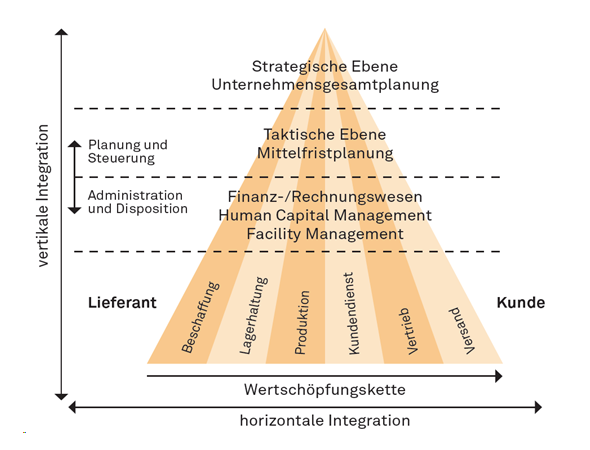
\includegraphics[width=\linewidth]{content/images/integrations-pyramide}\
    \quelle\url{http://www.referenzportal.ch/fuehrung/vom-erp-zum-integrierten-informationssystem/}
    \caption[Darstellung einer typischen Integrations-Pyramide]{Darstellung einer typischen Integrations-Pyramide\\}
    \label{fig:integrations-pyramide} 
\end{figure} 
Das Bild zeigt eine typische Integrations-Pyramide eines Unternehmens. In dieser Pyramide ist zum einen ersichtlich, dass für die Wertschöpfungskette die horizontale Integration wichtig ist, zum anderen jedoch auch, dass mehrere Abteilungen eines Unternehmens in einer Wertschöpfungskette durchlaufen werden müssen.
\\\\
Die Dauer zum durchlaufen der Wertschöpfungskette nennt man auch Time-to-Market. Wird die Kette in möglichst geringer Zeit durchlaufen, wird hierdurch die Time-to-Market Zeitspanne verringert.

\section{Begriffsabgrenzung}
\label{sec:Begriffsabgrenzung}

\subsection*{SOA und "`Service-orientierte Architektur"'}
Sowohl SOA als auch Microservices zählen zu dem Paradigma der "`Service-orientierten Architekturen"'.

Die Abkürzung SOA wird hier sowohl für das Paradigma "`Service-orientierte Architektur"' verwendet, wie auch für die spezielle Herangehensweise.

Um die beiden Thematiken in dieser Arbeit abzugrenzen wird der Begriff "`SOA"' für die Herangehensweise verwendet und die ausgeschriebene Variante zur Kennzeichnung des allgemeinen Paradigmas.

%\subsection*{Microservice}
%Der Begriff Microservice wird einerseits zum Beschreiben eines Architekturmodells genutzt, als auch zum beschreiben von eigenständigen Diensten (Services).

%Damit keine Verwechslung entsteht, wird in dieser Arbeit der Begriff "`Microservice"' verwendet, sofern das Architekturmodell gemeint ist und der Begriff "`Dienst"' oder "`Service"', wenn ein eigenständiger Dienst gemeint ist.

\section{Motivation}
\label{sec:motivation}
Die Anforderungen an Software werden zunehmend komplexer. Diese muss nicht nur funktionieren, sondern muss zum Teil in kürzester Zeit erweitert oder geändert werden, was eine besondere Herausforderung dar stellt. Dabei spielen sowohl funktionale, als auch nicht funktionale Anforderungen eine wichtige Rolle. Je komplexer Software wird, desto schwieriger ist sie zu warten und zu pflegen. 

\begin{quotation}
\frqq Die Zeitspanne des Time-to-Market [(TTM)] kann [dabei] ein sehr bedeutsamer Faktor für den Erfolg des Unternehmens darstellen und ist daher nicht zu vernachlässigen. Kurze Entwicklungszeiträume bei der Time-to-Market garantieren dem Unternehmen nämlich einen Vorteil gegenüber der Konkurrenz. Hier geht es darum, dem Kunden so schnell wie möglich ein neues und innovatives Produkt anbieten zu können.
    
Um den Erfolg durch eine kurze Time-to-Market zu unterstützen und zu fördern, investieren Unternehmen in ihre Entwicklungsabteilungen. Diese können sich so nur auf ihre jeweiligen Bereiche konzentrieren. Durch eine leistungsfähige Entwicklungsabteilung kann so, in Kombination mit einem gut organisierten Projektplan und eindeutigen Zuständigkeiten, die Zeitspanne Time-to-Market so klein wie möglich gehalten werden. Gerade in Branchen, in denen Innovation eine übergeordnete Rolle spielt und der Produkt-Lebens-Zyklus generell eher kurz ausfällt, spielt eine kurze Time-to-Market eine außerordentlich wichtige Rolle.\flqq \cite{ttm}
\end{quotation}

Zusätzlich entstehen Kosten für die Planung und Entwicklung des Produktes. Bis zur Veröffentlichung des Produktes hat das Unternehmen Geld und Zeit investiert. Je länger die Zeitspanne des TTM ist, umso erfolgreicher muss das Produkt sein, bzw. der Preis hoch genug sein. Daher muss die Zeitspanne des TTM möglichst gering gehalten werden, damit möglichst zeitnah die Schwelle, ab der die Erlöse und die Produktionskosten gleich hoch sind (Break-even-Point) erreicht wird. Die Time-to-Markt Zeitspanne beschreibt dabei die Zeit, in der die Wertschöpfungskette durchlaufen wird. Indem diese in möglichst geringer Zeit durchlaufen wird, wird die TTM-Zeitspanne gering gehalten. Jedes Unternehmen strebt daher eine kurze TTM Zeitspanne an.
\\\\
Zudem gibt es in einem Unternehmen nicht nur ein Softwareprodukt, sondern eine Vielzahl verschiedener Produkte für unterschiedliche Anwendungsfälle. Dabei kann es passieren, dass einige Anwendungen gleiche Funktionalitäten beinhalten. Müssen solche Funktionalitäten geändert werden, müssen dafür alle Anwendungen, welche diese Funktionen bereitstellen, geändert werden. Einfacher ist es daher, nur eine Anwendung zu haben, welche diese Funktionalität anbietet. Dadurch bedarf es nicht mehr der Anpassung von vielen Anwendungen, sondern nur noch von dieser einen.

\section{Ausgangssituation}
\label{sec:ausgangssituation}
Bei der Ausgangssituation handelt es sich um ein fiktives Szenario, welches an ein reales Problem angelehnt ist.
\\\\
Das Unternehmen \textit{Auktionen GmbH}\ ist ein modernes und aktives Internet-Unternehmen, welches seit 1995 existiert. Wie aus dem Namen zu entnehmen, betreibt das Unternehmen eine Auktionsplattform im Internet. Diese wurde zunächst als monolithische Anwendung implementiert.
\\\\
Mit zunehmenden Nutzerzahlen und damit täglichen Benutzungen, stellte das Unternehmen fest, dass es zunehmend schwieriger wurde, auf das Verhalten der Nutzer in angemessener Zeit zu reagieren. Da die zentrale Anwendung ein monolithisches System war, war es zudem schwierig diese zu deployen.
\\\\
Muss eine neue Version herausgebracht werden, so bedeutet dies entweder die gesamte Infrastruktur für Wartungszwecke offline zu nehmen und die Anwendung neu zu deployen oder Server im Parallelbetrieb laufen zu lassen und jeden neuen Besucher auf die neue Version zu leiten. Die letzte Methode bietet jedoch einige Schwierigkeiten, denn es könnten Änderungen eingebaut worden sein, welche im Konflikt mit der alten Version stehen. Dann muss in jedem Fall die erste Variante gewählt werden und die gesamte Infrastruktur offline genommen werden.
\\\\
Beide Varianten der Produktivname von Änderungen sind jedoch zeitaufwendig und komplex. Nicht nur das Deployen könnte Probleme bereiten, sondern auch die darauf folgende Ausführung des Programms. Wird der Code in einer monolithischen Applikationen geändert, kann dies ebenfalls Auswirkungen auf bestehende Teile des Codes haben, welche vorher, ohne Probleme, funktionierten. Werden Tests vernachlässigt oder wird nicht ausreichend getestet, kann es leicht passieren, dass sich Fehler einschleichen, wodurch eine Version in Betrieb genommen wird, welche Fehler enthält. Darauf folgend müssten diese behoben werden und die Anwendung erneut deployed werden.
\\\\
Im Falle einer monolithischen Architektur bedeutet das viele Änderungen für neue Features. Oft passiert es daher, dass Codestücke zurückbleiben, welche nicht mehr benötigt werden. Irgendwann ist die Applikation daher so groß, dass sie nicht mehr wartbar ist und neue Features nur noch schwer zu implementieren sind. Entstehen Fehler in solch einer Anwendung ist es umso schwerer diese zu finden und zu beheben.
\\\\
Aus diesem Grund hat die \textit{Auktionen GmbH} sich entschlossen, die monolithische Strukturen nicht weiter zu entwickeln, sondern auf eine Service-orientierte Architektur umzustellen.

\section{Vorgehen und Kapitel}
\label{sec:vorgehen}
Zunächst werden die Probleme bei der Verwendung von monolithischen Architekturen, unter dem Aspekt der Softwareentwicklung und Wartung analysiert. Darauf aufbauend soll die grundlegende Problematik herausgearbeitet werden. Anschließend werden die Grundlagen zur Verwendung von Service orientierten Architekturen und deren Vorteile, aufbauend auf die zuvor erläuterte Problematik, erklärt.
\\
Darauf folgend wird zunächst das Architekturparadigma "`SOA"' und anschließend das "`Microservice"' Paradigma betrachtet. Beide Paradigmen werden einzeln und unabhängig voneinander erläutert, um die spezifischen Eigenschaften beider Herangehensweisen herauszuarbeiten.
\\
Abschließend werden die gewonnen Kenntnisse zusammengetragen und ausgewertet. Dabei sollen beide Architekturparadigmen verglichen und bewertet werden. Zuletzt wird das Thema noch einmal zusammengefasst und ein Ausblick auf kommende Projekte bzw. die Bachelorarbeit gegeben.

\chapter{Problemanalyse}
\label{chap:analyse}
Jedes Internet-Unternehmen fängt klein an und wächst mit der Zeit. In dieser Zeit muss das Unternehmen viele Probleme bewältigen. Es muss die Produkte, welches das Unternehmen verkauft, weiterentwickeln und auf die Bedürfnisse der Nutzer reagieren. In unserer heutigen Zeit, in der das Internet das bevorzugte Informationsmedium ist, können sich Nutzer sehr schnell von einem Produkt zu einem anderen wechseln. Um das zu verhindern, muss ein Produkt immer aktuell sein.

\section{Herkömmliche Produkte}
Herkömmliche Software-Produkte wurden auf CDs/DVDs verkauft und änderten sich daher nie. Um ein aktuelles Produkt zu erhalten, musste die Software in einer aktuellen Version erworben werden und auch diese änderte sich dann nicht. Ggf. wurden Patches zu einem billigeren Preis angeboten, wodurch eine Software geändert und mit neuen Features ausgestattet werden konnte.

Die Informationen welche den Nutzern zur Verfügung standen war außerdem sehr gering, wodurch ein Produktwechsel selten war. Durch die kosten, welche aufgewandt werden mussten, um ein Produkt zu kaufen, war es sehr selten, dass Nutzer sich schnell entschieden ein anderes Produkt zu nutzen.

\section{Derzeitige Produkte}
Wie bereits erwähnt ist das Internet das heute bevorzugte Medium, um Informationen über Produkte und andere Dinge zu erhalten. Nutzer können innerhalb von Minuten Produkte vergleichen und durch Demos diese testen, meistens sogar mit vollem Funktionsumfang. Durch SaaS (Software-as-a-Service) ist auch das wechseln von Produkten nach dem "bezahlen" möglich, da man beim SaaS-Model nur das Zahlt, was man auch wirklich nutzt.

Aus genau diesen Gründen, muss sich ein Internet-Unternehmen sehr schnell anpassen und auf die Bedürfnisse der Nutzer reagieren. Schafft ein Unternehmen dieses nicht, kann es schnell dazuführen, dass es Insolvent wird.

\section{Aktuelles Beispiel: \ebay}
Ein Modernes und aktives Internet-Unternehmen ist \ebay und darf man der Seite \cite{highscalability} glauben, so startet die Seite 1995 als Monolithische Perl Applikation. Selbst wenn diese Informationen nicht auf \ebay zutreffen sollten, so dient es uns doch als gutes Beispiel einer realen Problemstellung.

Laut Wikipedia (https://en.wikipedia.org/wiki/EBay) wurde \ebay 1995 von Pierre Omidyar unter dem Namen \textit{ActionWeb} gegründet und wurde 1997 in \ebay umbenannt. \ebay wurde wie oben schon angesprochen als Monolithische Perl Anwendung implementiert. Mit der Steigerung der Reichweite und der täglichen Benutzung, hatte man sich dann aber dazu entschlossen auf C++ als Code-Basis umzusteigen und die Seite mit CGI zu implementieren. Mittlerweile war \ebay ein großes und sich rasant entwickelndes Unternehmen. Das bedeutet aber auch, dass \ebay ständig auf das Verhalten der Nutzer reagieren und sich anpassen muss. Man versuchte also eine Monolithische Applikation mit der Fähigkeit auszustatten, auf Änderungen schnell zu reagieren, implementieren und deployen. Aber ein Monolith zu deployen, bedeutet, entweder die gesamte Infrastruktur für Wartungszwecke offline zu nehmen und die Applikation neu zu deployen, oder Server im Parallel betrieb laufen zu lassen und jeden neuen Traffic auf die neue Version zu routen. Die letzte Methode bietet jedoch einige Schwierigkeiten, denn es könnten Änderungen eingebaut worden sein, welche im Konflikt mit der alten Version stehen. Dann muss in jedem Fall die erste Variante gewählt werden und die gesamte Infrastruktur offline genommen werden.

Beide Varianten der Änderungen sind jedoch zeitaufwendig und  schwierig, denn nicht nur das deployen könnte Probleme bereiten, sondern auch die darauf folgende Ausführung des Programms. Ändert man Code in Monolithischen Applikationen kann das auch Auswirkungen auf bestehende Teile des Codes haben, welche vorher, ohne Probleme, funktioniert haben. Werden Tests vernachlässigt oder wird nicht ausreichend getestet, kann es leicht passieren, dass sich ungewollt Fehler einschleichen, wodurch dann eine Version in betrieb genommen wird, welche Fehler enthält. Darauf folgend müssten diese wieder behoben werden und die Anwendung erneut deployed werden.

Im Falle einer Monolithischen Architektur bedeutet das viele Änderungen und neue Features. Oft passiert es daher, dass Code Stücke zurückbleiben, welche nicht mehr benötigt werden. Irgendwann ist die Applikation daher so groß, dass sie nicht mehr Wartbar ist und neue Features nur noch schwer zu implementieren sind. Entstehen Fehler in solch einer Anwendung ist es um so schwerer diese zu finden und zu beheben. Schließlich hat sich \ebay entschlossen ihre "Anwendung" in Java neu zu implementieren. Dieses mal jedoch mit dem Hintergrund einer leicht erweiterbaren und wartbaren Architektur.

\section{Das Problem}
Das Problem besteht also darin, "eine Anwendung" flexibel und einfach erweiterbar zu gestalten, damit ein Unternehmen schnell auf Änderungen und die veränderten Bedürfnisse der Nutzer reagieren kann. Damit solch eine Software ebenfalls gut Wartbar ist, sollten Redundanzen möglichst vermieden werden. Hier steigen wir in Modularität ein, denn damit eine Software möglichst einfach Wartbar ist, sollte jeder Code mit einem bestimmten Kontext in ein eigenes Modul gepackt werden. So können zum Beispiel alle Codestücke einer bestimmten Berechnung in ein Modul gepackt werden, wodurch diese dann nur an einer zentralen Stellen geändert werden muss. Wenn die Module jedoch auch von verschiedenen Applikationen genutzt werden, müssen diese in Libraries ausgelagert werden. Auch hier hat man wieder nur eine zentrale Stelle, an der Änderungen vorgenommen werden müssen, um die Berechnung anzupassen oder zu ändern. Jedoch besteht hier das Problem, dass wenn Änderungen durchgeführt werden, diese noch lange nicht in jeder laufenden Applikation zu finden sind. Dazu müssen diese nämlich erst einmal neu gebaut und deployed werden, damit diese Produktiv werden.

Um dieses Vorgehen zu vereinfachen hat man sich dazu entschieden, diese Libraries in eigene Applikationen (Services) zu verpacken und diese über eine Schnittstelle anzubieten. Das sorgt dafür, dass jede Software, welche dieses Modul benötigt, sie nicht mehr eigenständig implementieren muss, sondern den dafür vorgesehenen Service aufrufe kann, um die nötigen Informationen zu erhalten. Diese Services werden auch als Microservices bezeichnet, da sie nur einem bestimmten Zweck dienen, dafür ihre Aufgabe aber besonders gut erledigen. Hierbei kann man unter anderem von einer \SOA\ (SOA) sprechen. Es sollte jedoch darauf geachtet werden, dass weder zu viel, noch zu wenig in ein Service gepackt wird. Welche Größe genau richtig ist, wird im Kapitel \secref{chap:grundlagen} weiter erläutert.

\section{Herausforderung}
Bevor ein Programm entwickelt werden kann, müssen verschiedene Schritte durchlaufen werden. Es muss zunächst ein bedarf für die Software bestehen. Sei es Unternehmens-Software, welche eingesetzt wird um eine bestimmte Aufgabe zu erledigen oder aber um eine neue Technologie zu testen, ohne das diese Produktiv eingesetzt wird. Im jeden Fall benötigt man ein Kontext für das zu entwickelnde Programm und damit auch die Anforderungen an dieses. Nach dem erfassen dieser, muss die interne Architektur der Software geplant und schließlich umgesetzt werden. 

Oft passiert es, das ein Unternehmen große Vorstellungen von dem Unternehmens-Ziel hat. Dies führt häufig dazu, dass Software entwickelt wird, welches weit über den aktuellen Anforderungen hinaus gehen. Man möchte damit verhindern, Software an einem späteren Zeitpunkt neu zu entwickeln oder austauschen zu müssen. Jedoch kann dies zu großen Problemen führen sobald das Unternehmen wächst und den am Anfang genannten Vorstellungen näher kommt. In dieser Phase entstehen meistens Probleme, welche vorher nicht berücksichtigt worden sind, weil niemand sie kannte. Dadurch muss die vorhandene Software, welche eigentlich für dieses Szenario ausgelegt war, geändert werden.
%Time-to-Market
Das selbe gilt, wenn man eine Architektur verwenden möchte, mit der man nicht vertraut ist. Wer zum Beispiel wenig mit Microservices und \SOA\ (SOA) gearbeitet hat, aber es trotzdem verwenden möchte, weil es die Probleme lösen kann, welche später auftreten könnten, muss damit rechnen, dass 



\chapter{Grundlagen}
\label{chap:grundlagen}

\section{Architektur}


\chapter{Microservices}
\label{chap:Microservices}

\section{Überblick}
\label{sec:überblickMicroservice}
"Modularisierung ist nichts Neues. Schon lange werden große Systeme in kleine Module unterteilt, um Software einfacher zu erstellen, zu verstehen und weiterzuentwickeln. Das Neue: Microservices nutzen als Module einzelne Programme, die als eigene Prozesse laufen. Der Ansatz basiert auf der UNIX-Philosophie. Sie lässt sich auf drei Aspekte reduzieren:"\cite[S. 2]{EWolff2016:Microservices}

\begin{itemize}
    \item Ein Programm soll nur eine Aufgabe erledigen, und das soll es gut machen.
    \item Programme sollen zusammenarbeiten können.
    \item Nutze eine universelle Schnittstelle. In UNIX sind das Textströme.
\end{itemize}
Diese Art der Aufteilung wurde schon lange von großen Unternehmen wie Amazon oder Google genutzt und wurde zu nächst \SOA (SOA) genannt. Jedoch unterscheiden sich Microservices und SOA voneinander. Daher wird SOA im Nächsten Kapitel genauer erläutert und im Kapitel \ref{chap:ergebnisse} die Ergebnisse zusammen gefasst und beide Technologien mit einander verglichen.
\\\\
Der Begriff Microservices ist nicht eindeutig definiert. Als erste Näherung dienen, nach Eberhard Wolff \cite[S. 2]{EWolff2016:Microservices}, folgende Kriterien:

\begin{itemize}
    \item Microservices sind ein Modularisierungskonzept. Sie dienen dazu. ein großes Software-System aufzuteilen - und beeinflussen die Organisation und die Software-Entwicklungsprozesse.
    \item Microservices können unabhängig von Änderungen an anderen Microservices in Produktion gebracht werden.
    \item Microservices können in unterschiedlichen Technologien implementiert sein. Es gibt keine Einschränkung auf eine bestimmte Programmiersprache oder Plattform.
    \item Microservices haben einen eigenen Datenhaushalt: eine eigene Datenbank - oder ein vollständig getrenntes Schema in einer gemeinsamen Datenbank.
    \item Microservices können eigene Unterstützungsdienste mitbringen, beispielsweise eine Suchmaschine oder eine spezielle Datenbank. Natürlich gibt es eine gemeinsame Basis für alle Microservices - beispielsweise die Ausführung virtueller Maschinen.
    \item Microservices sind eigenständige Prozesse - oder virtuelle Maschinen, um auch die Unterstützungsdienste mitzubringen.
    \item Dementsprechend müssen Microservices über das Netzwerk kommunizieren. Dazu nutzen Microservices Protokolle, die lose Kopplung unterstützen. Das kann beispielsweise REST sein - oder Messaging-Lösungen.
\end{itemize}
Obwohl der Begriff nicht eindeutig definiert ist, liegt jedoch bei jedem Service-orientierten Systemen, ein Verteiltes System zu Grunde und auch die damit verbundenen Probleme und Herausforderungen.

\section{Gr"o\ss e von Microservices}
\label{sec:groesseMicroservice}
"Der Name \frqq Microservices\flqq\ verrät schon, dass es um die Servicegröße geht - offensichtlich sollen die Services klein sein."\cite[S. 31]{EWolff2016:Microservices} Es gibt verschiedene Möglichkeiten die Größe von Programmen zu ermitteln. Eine Variante ist zum Beispiel das Zählen von  Lines of Code (LOC), jedoch hat diese Methode auch Nachteile. Denn die Anzahl der Codezeilen hängen stark von der verwendeten Programmiersprache ab. Einige Programmiersprachen benötigen mehr Zeilen Code, um eine bestimmte Tätigkeit abzubilden, als andere.
\\
Die Größe von Services sollte jedoch nicht von zentraler Bedeutung sein, denn eine untere Grenze gibt es für Services nicht. "Wohl aber eine obere Grenze: Wenn der Microservice so groß ist, dass er von einem Team nicht mehr weiterentwickelt werden kann, ist sie zu groß. Ein Team sollte dabei eine Größe haben, wie sie für agile Prozesse besonders gut funktioniert. Das sind typischerweise drei bis neun Personen."\cite[S. 34]{EWolff2016:Microservices}
\\
Bei der Größe eines Services ist jedoch darauf zu achten, das ein Service nicht zu viele oder zu wenige Funktionen besitzt. Wie bereits beschrieben, sind Microservices modulare, lose gekoppelte Services. Wird ein Service zu klein angesetzt, können daraus Abhängigkeiten zu anderen Services entstehen und damit das gesetzt der losen Kopplung verletzten. Besitzt hingegen ein Service zu viele Funktionen, wird es meistens nicht mehr als Microservice angesehen, da es nicht eine, sondern mehrere Aufgaben übernimmt und diese wahrscheinlich nicht mehr gut erledigen kann.

\section{Orchestration vs Choreographie}
\label{sec:orchestrationvschoreographie}
Möchte man ein Microservice System aufbauen, stellt sich immer wieder die Frage, wie einzelne Services Strukturiert werden und wie diese unter einander kommunizieren sollen. Ein bestimmter Vorgang startet in der Regel bei einem Service. Nun muss man entscheiden ob weitere Services hinzugezogen, beziehungsweise informiert werden müssen. Je nach Anwendungsfall muss man sich zwischen Service Orchestration und Choreographie entscheiden. Dabei ist es fast unmöglich ein ganzes Microservice-System aus nur einem der beiden Varianten zu bauen.

\subsection{Orchestration}
\label{subsec:orchestration}
Bei der Orchestration handelt es sich um eine Komposition von Services. Ein Geschäftsprozess wird zwar mit Hilfe von mehreren Services abgebildet, jedoch ist nur ein Service dafür zuständig den Geschäftsprozess durchzuführen.
\newpage
\begin{figure}[htb]
    \centering 
    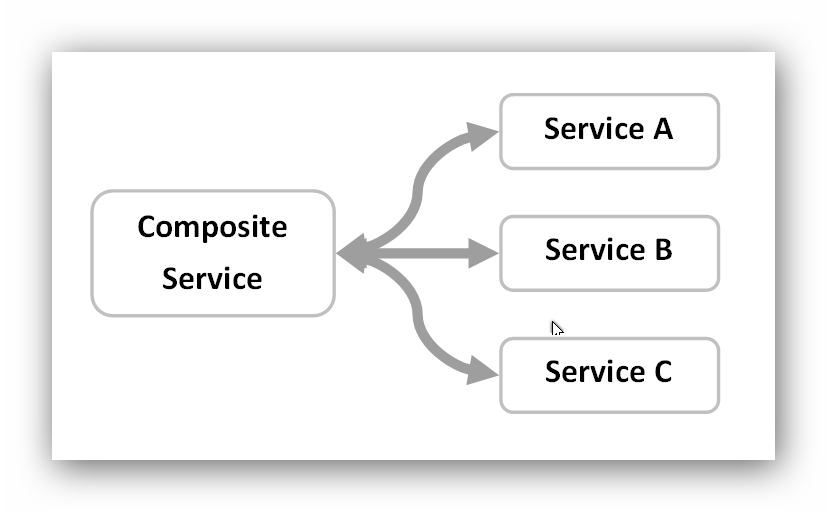
\includegraphics[width=\linewidth]{content/images/ServiceOrchestration}\
    \caption[Orchestration]{Orchestration}
    \label{fig:ServiceOrchestration}  
\end{figure}
\noindent
Wie die Abbildung zeigt besteht \textbf{\underline{keine}} Verbindung zwischen:
\begin{itemize}
    \item A \& B
    \item A \& C
    \item B \& C
\end{itemize}
Nur der "`Composite Service"' nutzt die anderen Microservice um den Geschäftsprozess abzubilden. Diese Art der Kommunikation nennt man Orchestration und wird im Kapitel \secref{chap:soa} noch einmal behandelt.

\subsection{Choreographie}
\label{subsec:choreographie}
Anders als bei der Orchestration können Microservices bei der Choreographie beliebig untereinander kommunizieren. Das ist vor allem dann Sinnvoll, wenn verschiedene Microservice andere Microservice über Änderungen oder andere Aktionen informieren müssen.

\begin{figure}[htb]
    \centering 
    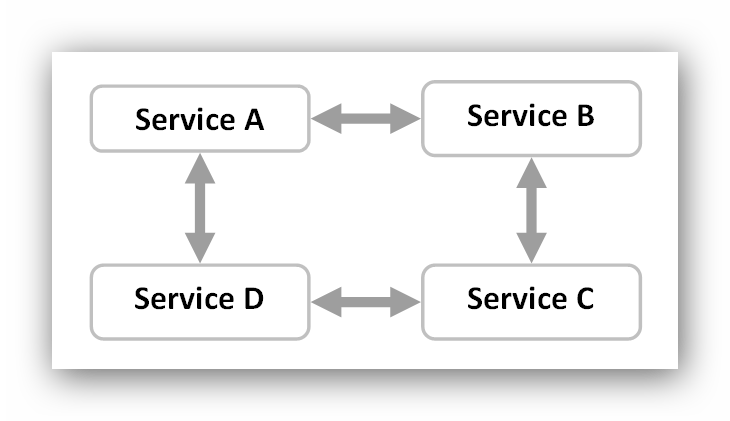
\includegraphics[width=\linewidth]{content/images/ServiceChoreography}\
    \caption[Choreographie]{Choreographie}
    \label{fig:ServiceOrchestration}  
\end{figure}

% [Seite 66 EWolff2016] Technologische Wahlfreiheit
\subsection{Herausforderung}
\label{sec:Herausforderung}
Wie bereits in \secref{sec:überblickMicroservice} erwähnt, liegt ein Verteiltes System zu Grunde und damit auch die Grundlegenden Probleme der Kommunikation (siehe \cite[S. 25]{EWolff2016:Microservices}).
Der Ausfall eines Services kann im schlechtesten Fall dazu führen, dass alle anderen Microservices nicht mehr funktionieren. Um das zu verhindern muss klar definiert werden, was Microservices in dieser Situation tun sollen. Zusätzlich muss, sofern Datenbank Operationen eine wichtige Rolle Spielen, das Problem der einheitlichen Transaktion gelöst werden. Wenn zum Beispiel eine Operation Daten über verschiedene Microservices in Datenbanken schreibt, muss bei nicht Erreichbarkeit oder Fehlers eines Microservices eine einheitlicher Rollback durchgeführt werden, um keine inkonsistente Dateien im System zu haben.
Eine weitere Herausforderung besteht in dem Grundkonzept von Microservices. Da nicht definiert ist, welche Programmiersprache für Microservices verwendet wird, kann ein Service zum Beispiel in Java, ein anderes in Scala ode Python geschrieben werden. Es muss daher dafür gesorgt werden, dass die einzelnen Services untereinander interoperabel sind. Um das zu gewährleisten, müssen die Schnittstellen möglichst einheitlich und auf dem gleichen Protokoll aufbauend programmiert werden. Hier bieten REST-Schnittstellen eine gute Lösung. Diese können auf dem HTTP-Protokoll aufgebaut werden. Zusätzlich bietet das HTTP-Protokoll die Möglichkeit, ein einheitliches Medium, wie zum Beispiel XML oder JSON, als Informationsträger zu nutzen. Dabei kann theoretisch jeder Microservice mit jedem anderen Microservice kommunizieren, sofern die Schnittstellen einheitlich definiert sind.

\section{PUSH- VS PULL-Architektur}
\label{sec:PushPullArchitektur}
Grundlegend können Microservices mit Hilfe zwei verschiedener Kommunikations-Architekturen kommunizieren, PUSH- und PULL-Architektur. Dabei ist jedoch nicht ausgeschlossen, dass sobald eine Architektur gewählt worden ist, die andere nicht mehr genutzt werden kann. Genauso wie bei der Entscheidung über die Kommunikationsstruktur (siehe \secref{subsec:orchestration}), kann es von Vorteil sein, beide Architekturen zu nutzen.
\\\\
\textbf{PULL-Architektur}\\
Eine PULL-Architektur basiert auf einen einfachen Request-Replay-Schema. Dementsprechend ist das Web PULL-basiert.
Der Browser macht eine Anfrage an einen Server, dieser wiederum verarbeitet die Anfrage und liefert eine Antwort (Replay) zurück. Dies hat den Vorteil, das nicht lange auf eine Antwort gewartet werden muss und die teilhabenden Kommunikationspartner gegenseitig kennen, jedoch bringt es auch den Nachteil, dass dadurch weitgehend eine synchrone Kommunikation stattfindet und eine Antwort häufig nicht gleichzeitig an mehrere Empfänger senden kann.
\\\\
\textbf{PUSH-Architektur}\\
Eine PUSH-Architektur wird eingesetzt, wenn man verschiedene Kommunikationspartner über bestimmte Ereignisse informieren möchte. Hier stehen meist nicht die Kommunikationspartner, sondern die Informationen im Vordergrund. Dafür wird meistens ein eigenständiger Service (Broadcaster) eingesetzt, der die Verteilung dieser Informationen übernimmt. Dabei kann ein Service als Informationsprovider dienen, zum Beispiel ein Nachrichten-Feed (Von einer Nachrichtenseite). Alle anderen Services abonnieren den Broadcaster und erhalten dadurch alle Nachrichten, die der Informationsprovider sendet.
Es gibt jedoch auch den Fall, dass die Kommunikation sternförmig um den Broadcaster angeordnet sind. Dadurch ist jeder Service der diesen abonniert, sowohl Provider, als auch Consumer.
Anders als bei PULL-basierten Systemen kann hier nicht unbedingt sichergestellt werden, dass alle Nachrichten von allen Konsumern gleichzeitig gelesen und ggf. verarbeitet werden. Jedoch können so Informationen innerhalb eines Microservice-Systems relativ zuverlässig verteilt werden.
Der Vortiel von PUSH-Architekturen ist, dass eine asynchrone Informationsverbreitung aufgebaut werden kann. Zudem können Serviceausfälle, solange es nicht der Boradcaster oder wichtige Microservices sind, überbrückt werden, indem der Broadcaster die Nachrichten für eine bestimmte Zeit vorhält und so der Microservice, welcher nicht erreichbar war, die Nachrichten trotzdem noch erhält.
\\\\
Oft ist es nicht notwendig eine Antwort zu erhalten. Zum Beispiel muss eine Registrierung in unserem fiktiven Unternehmen, der \gmbh\ möglich sein. Dabei sendet der Microservice der für die Registrierung zuständig ist eine einfache Event-Nachricht, wie Benutzer XY hat sich Registriert. Im Hintergrund kann dann zum Beispiel ein anderer Microservice diese Nachricht erhalten und zusätzliche Aktionen durchführen, wie erstellen des Warenkorbs.

\section{Continuous-Delivery}
\label{sec:ContinuousDelivery}
"Wer bisher nur Deployment-Monolithen betrieben hat, ist bei Microservices damit konfrontiert, dass es sehr viel mehr deploybare Artefakte gibt, weil jeder Microservice unabhängig in Produktion gebracht wird"\cite[S. 241]{EWolff2016:Microservices}
"Unabhängiges Deployment ist ein zentrales Ziel von Microservices. Außerdem muss das Deployment automatisiert sein, weil ein manuelles Deployment oder auch nur manuelle Nacharbeitung aufgrund der großen Anzahl Microservices nicht umgesetzt werden können"\cite[S. 256]{EWolff2016:Microservices}

\chapter{\SOA\ (SOA)}
\label{chap:soa}

\section{Architektur}
\label{sec:SoaArchitektur}

\section{EnterpriseServiceBus - ESB}
\label{sec:esb}


% [Seite 69 EWolff2016] Vergleich Google/Alphabet
\section{Vergleich}


% ***************************** BIBLIOGRAPHY **********************************
\baselineskip=14pt
\addcontentsline{toc}{chapter}{\protect\numberline{}\bibname}
\bibliography{bib/thesis}

% ******************************* APPENDIX ************************************
\appendix
\baselineskip=18pt
\chapter{Diagramme und Tabelle}
\label{chap:anhang_a}


\end{document}
